\section{Introduction} \label{RSS:sec:introduction}

In recent years, interest in applying deep learning to robotic manipulation has increased. However, the lack of cheap data has proven to be a significant limitation \cite{DisbandOpenAI2021}. To enable applications such as smart and flexible manufacturing, logistics, and care-giving robots \cite{WEFRobots}, we must develop methods that learn from smaller datasets, especially if the learning is done online on real robots.

One of the simplest and most effective ways to mitigate the problem of small datasets is to use data augmentation. While data augmentation has been shown to significantly improve generalization performance in tasks like image classification, it is not straightforward to extend existing data augmentation methods to the types of data used in robotic manipulation. Furthermore, most existing augmentation methods fall into one of two categories, and both have severe limitations:

In the first category, augmentations are defined by a set of transformations, sampled independently for each example. Most image augmentation methods fall into this category, where rotations or crops are sampled randomly for each example \cite{Augerino2020,AutoAugment,BestPractice2003}. By making augmentations independent of the example being augmented, we are restricted to operations which are valid on all examples. In the second category, there are methods which learn a generative model (VAE, GAN, etc.) of the data, and then sample new training examples from that model \cite{BayesianDATran2017,MaterialsAEOhno2020,PriceForecastingAE2021}. This approach assumes a useful generative model can be learned from the given dataset, but we found these methods did not perform well when the dataset is small.

\begin{figure}
    \centering
    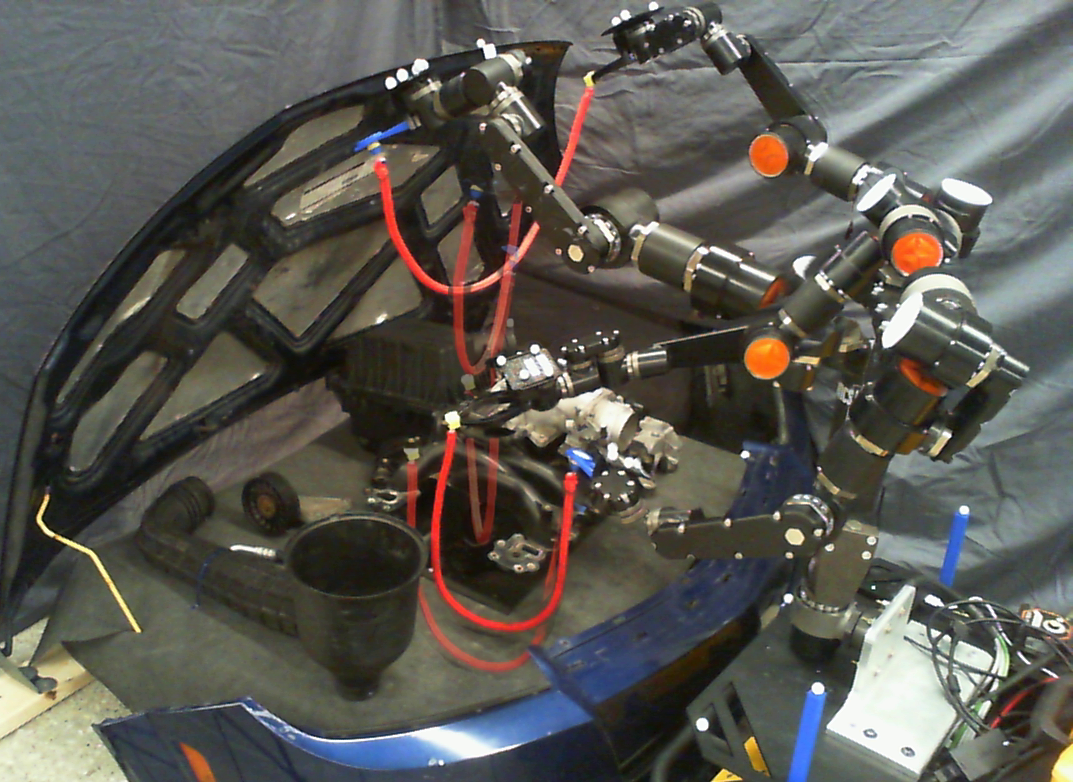
\includegraphics[width=0.9\linewidth]{Chap3/images/title_figure.png}
    \caption{A mock-up of a car engine bay. The robot must move the rope and place it under the engine without snagging it to set up for lifting the engine. We use data augmentation to improve task success rate during online learning for this task.}
    \label{RSS:fig:real_robot_setup}
\end{figure}

\begin{figure*}
    \centering
    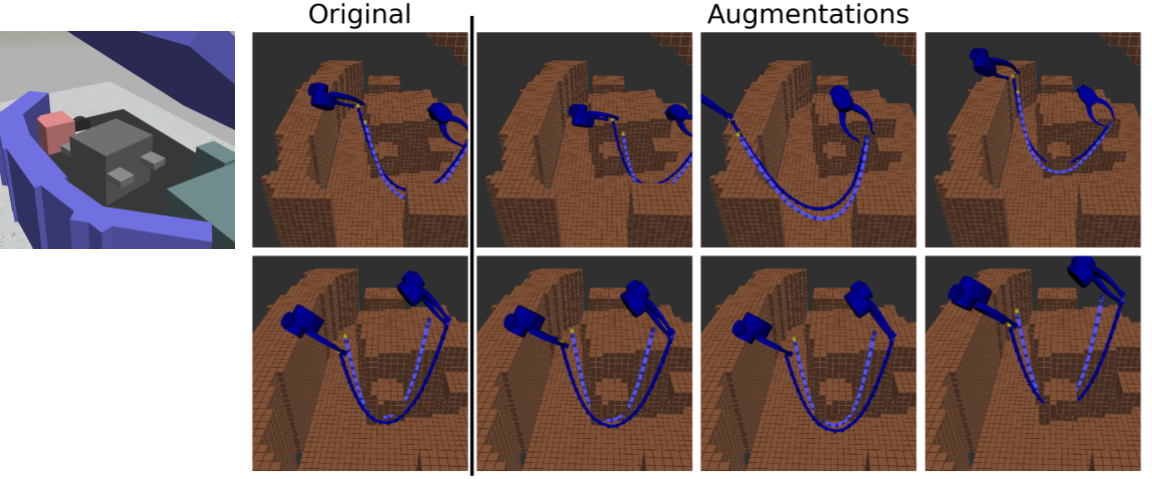
\includegraphics[width=1\linewidth]{Chap3/images/rope_aug_examples.png}
    \caption{Examples of augmentations of rope generated by our method. On the left is a picture of the scene in simulation from a zoomed out viewpoint. The simplified engine block model is in the center. The rope start (dark blue) and end (light blue) states are shown, with the grippers shown at the start state. The static environment geometry is shown in brown. The first row shows a transition in free space, where the resulting augmentations are particularly diverse. The final augmentation shows how our method found a transformation to move the rope underneath the hook while remaining in free space. The second row shows a transition which involves contact between the rope and the environment. The augmentations preserve this contact.}
    \label{RSS:fig:rope_aug_examples}
\end{figure*}


It is not trivial to define a coherent framework for data augmentation that encompasses many domains and many types of learning problems (e.g. classification and regression). Thus, the first contribution of this chapter is a formalization of the data augmentation problem. In our problem statement (Section \ref{RSS:sec:problem}), we formalize data augmentation as an optimization problem based on three key criteria: \textit{validity}, \textit{relevance}, and \textit{diversity}. We define an augmented example as \textit{valid} if it obeys the laws of physics and is possible in the real world. Augmentations are \textit{relevant} if they are similar to data that would be seen when performing the target task. \textit{Diversity} encourages the augmentations to be as varied as possible, i.e. the transformations applied to the data should be uniformly distributed to maximize diversity. Producing diverse augmentations for each original example is key to improving the generalization of the trained network.

The general definitions of validity, relevance, and diversity we propose depend on information that is intractable to compute for many manipulation problems, and therefore we also present approximations to these definitions. We do not claim that this formulation is useful for all manipulation problems, and clearly define the physical assumptions behind this formulation in Section \ref{RSS:sec:problem}.

Our second contribution is a method for solving this approximated optimization problem. Our method operates on trajectories of object poses and velocities, and searches for rigid-body transformations to apply to the moving objects in the scene to produce augmentations. Our method encourages validity by preserving contacts and the influence of gravity. Additionally, we encourage relevance by initializing the augmentations nearby the original examples and preserving near-contacts. Finally, we encourage diversity by pushing the augmentations towards randomly sampled targets.

Our results demonstrate that training on our augmentations improves downstream task performance for a simulated cluttered planar-pushing task and a simulated bimanual rope manipulation task. The learning problems in these tasks include classification and regression, and have high-dimensional inputs and outputs. Lastly, we demonstrate our augmentation in an online learning scenario on real-robot bimanual rope manipulation using noisy real-world perception data (Figure \ref{RSS:fig:real_robot_setup}). In this scenario, augmentation increased the success rate from 27\% to 50\% in only 30 trials. Additional materials such as code and video can be found on our \href{https://sites.google.com/view/data-augmentation4manipulation}{project website}.
